\documentclass{article}
\usepackage{graphicx}
\usepackage{amsthm}
\usepackage{amsfonts}
\usepackage{amsmath}
\usepackage{amssymb}
\usepackage{fullpage}
\usepackage[usenames]{color}
\usepackage{hyperref}
  \hypersetup{
    colorlinks = true,
    urlcolor = blue,       % color of external links using \href
    linkcolor= blue,       % color of internal links 
    citecolor= blue,       % color of links to bibliography
    filecolor= blue,        % color of file links
    }
    
\usepackage{listings}

\definecolor{dkgreen}{rgb}{0,0.6,0}
\definecolor{gray}{rgb}{0.5,0.5,0.5}
\definecolor{mauve}{rgb}{0.58,0,0.82}

\lstset{frame=tb,
  language=haskell,
  aboveskip=3mm,
  belowskip=3mm,
  showstringspaces=false,
  columns=flexible,
  basicstyle={\small\ttfamily},
  numbers=none,
  numberstyle=\tiny\color{gray},
  keywordstyle=\color{blue},
  commentstyle=\color{dkgreen},
  stringstyle=\color{mauve},
  breaklines=true,
  breakatwhitespace=true,
  tabsize=3
}

\theoremstyle{theorem} 
   \newtheorem{theorem}{Theorem}[section]
   \newtheorem{corollary}[theorem]{Corollary}
   \newtheorem{lemma}[theorem]{Lemma}
   \newtheorem{proposition}[theorem]{Proposition}
\theoremstyle{definition}
   \newtheorem{definition}[theorem]{Definition}
   \newtheorem{example}[theorem]{Example}
\theoremstyle{remark}    
  \newtheorem{remark}[theorem]{Remark}


\title{CPSC-406 Report}
\author{Everett Prussak  \\ Chapman University}

\date{\today}

\begin{document}

\maketitle

\begin{abstract}
Consisting of CPSC 406 Material at Chapman University with Professor Alexander Kurz. This report will include an Introduction, Weekly Homework, and a Paper on the group project, which is done throughout the semester. 
\end{abstract}

\tableofcontents

\section{Introduction}\label{intro}
This report...

\section{Homework}\label{homework}

This section contains solutions to homework. 

\subsection{Week 2 (Homework 1)}
This week's homework was to solve the following NFA:\noindent\newline
\includegraphics[scale=0.8]{a}\noindent\newline
\noindent\newline This is the following NFA but drawn out:

\includegraphics[scale=0.2]{nfa}\noindent\newline

From this NFA, the following DFA table can be made:\noindent\newline
\includegraphics[scale=0.8]{b}\noindent\newline

\includegraphics[scale=0.2]{dfa}\noindent\newline

\noindent\newline\newline This DFA diagram will allow for the correct initial state, final states, and correct path for each input.


\subsection{Week 3 (Homework 2)}
\noindent Week 3 consisted of 2 Questions. They are in their respective sections.\newline

\subsubsection{Question 1}
For Week 3 Question the object was to write the steps of the unification algorithm for each pair. \newline

\includegraphics[scale=0.75]{c}\noindent\newline

\noindent\newline For number 1 of question 1 I got the following answer:

\begin{verbatim}
1. f(X,f(X,Y)) = f(f(Y,a),f(U,b))

  1. X = f(Y,a)
      o1 = [f(Y,a)/X]

  2. f(X,Y) = f(U,b)
      3. X = U
          o3 = [U/X]
      4. Y = b
          o4 = [b/Y]

  5. X(o3 * o4) = U, f(o3 * o4)(Y,a) = f(b,a)
      U = f(b, a)
      o5 = [f(b,a)/U]


o = o3 * o4 * o5 = [U/X, b/Y, f(b,a)/U]
X = U, Y = b, U = f(b,a)
\end{verbatim}

\noindent\textbf{Note: Sigma Symbol was not working in Verbatim, thus a simple lowercase o was subsitituted.}

\noindent\newline\newline For number 2 of question 1 I got the following answer:

\begin{verbatim}
2. f(g(U),f(X,Y)) = f(X,f(Y,U))

  1. g(U) = X
       o1 = [g(U)/X]

  2. f(X,Y) = f(Y,U)
       3. X = Y
          o3 = [Y/X]
       4. Y = U
          o4 = [U/Y]

o = o1 * o2 * o3 = [X/U, Y/X, g(Y)/Y]
\end{verbatim}

\noindent\newline\newline For number 3 of question 1 I got the following answer:
\begin{verbatim}
3. h(U,f(g(V),W),g(W)) = h(f(X,b),U,Z)

  1. U = f(X,b)
     o1 = [f(X,b)/U]

  2. f(g(V),W) = U
     o2 = [f(g(V),W)/U]

  3. g(W) = Z
     o3 = [g(W)/Z]

  4. U(o1 * o2) --> f(X,b) = f(g(V),W)

     5. X = g(V)
        o5 = [g(V)/X]

     6. b = W
        o6 = [b/W]

  7. Z(o3 * o6) = g(W), W = b
     o7 = [g(b)/Z]

  8. U(o1 * o2 * o6) --> f(X,b) = f(g(V), b)
     o8 [f(g(V),b)/U]


  o = o5 * o6 * o7 * o8 = [f(g(V),b)/U, g(V)/X, b/W, g(b)/Z]


  U = f(g(V),b), W = b, X = g(V), Z = g(b)
\end{verbatim}

\subsubsection{Question 2}
For question 2, the task was to draw a SLD Recursion Tree for the following:\newline
\includegraphics[scale=0.65]{f}\newline\newline\newline

\noindent I got the following SLD Tree:
\begin{verbatim}



                   twoway(W,a)
                  /           \
                 /             \
              conn(W,a)        conn(a,W)
              /        \        /       \
            W=b        W=d   W=c       no
                        |            /  |  \
                        no          b   d   c
\end{verbatim}

\noindent\newline twoway(W,a) becomes conn(W,a) and conn(a,W) because of the rule twoway(X,Y):- conn(X,Y), conn(Y,X). This becomes the first part of the tree. Then for the conn(X,Y), it becomes conn(W,a). This side of the tree will split into W=b and W=d. W=d eventually fails because there is no serv(d). However, W=b is successful because we have addr(a,b) and a a serv(b), which allows for the conn(b,a) to be true. On the right side of the tree, we have conn(a,W). This will split into w=c and no. Since c holds the address of a, and b holds the address of c, and serv(b) exists, we can create a conn(a,c) because of these factors. We see in the equation addr(X,Z), serv(Z), addr(Z,Y) can be applied here. In our case it would look similar to addr(a,b) serv(b) addr(b,c), which allows conn(b,c) to be true.


\subsection{Week 6 (Homework 3)}
\noindent\newline The goal this week was to solve the following:

\includegraphics[scale=0.64]{abcd}\noindent\newline

\noindent\newline I split this into to two parts (Top and Bottom Questions).

\subsubsection{Part 1 (Top)}
\noindent\newline Here is my answer for number 1:

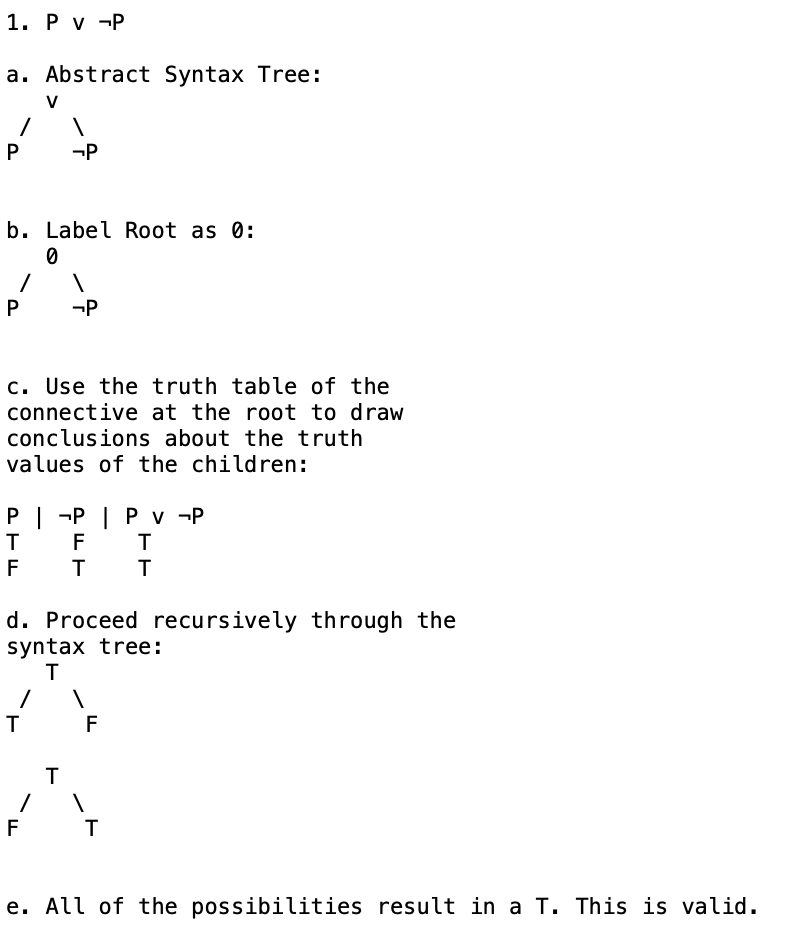
\includegraphics[scale=0.64]{hw6_1}\noindent\newline

\noindent\newline Here is my answer for number 2:

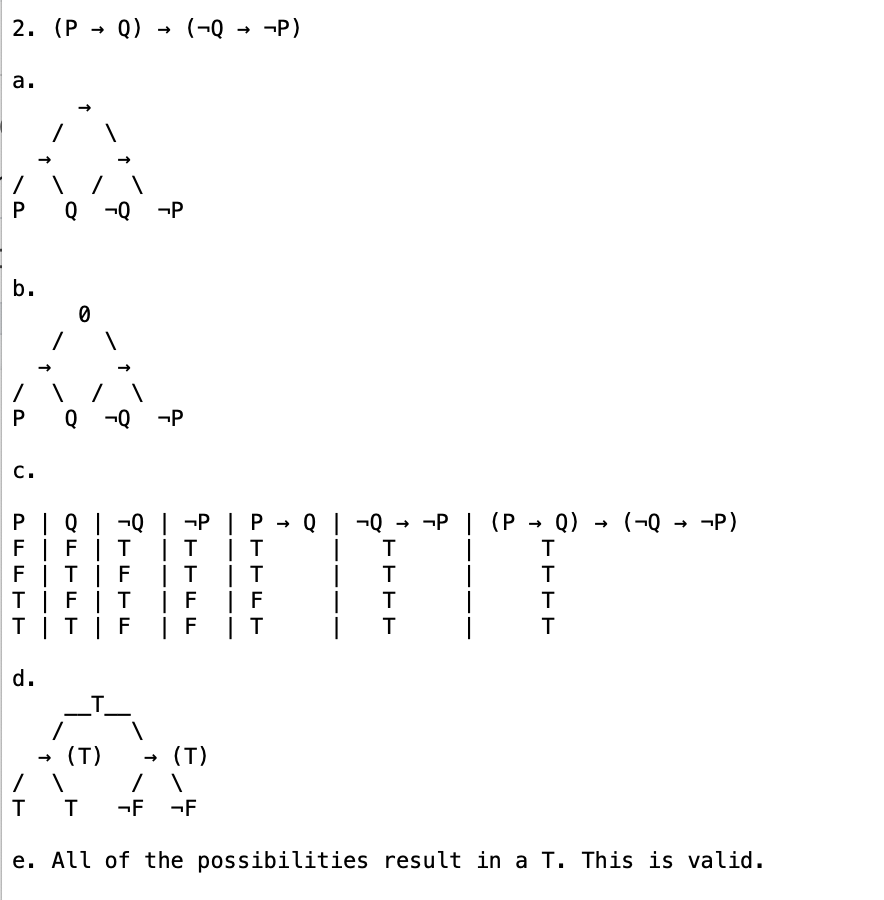
\includegraphics[scale=0.64]{hw6_2}\noindent\newline

\noindent\newline Here is my answer for number 3:

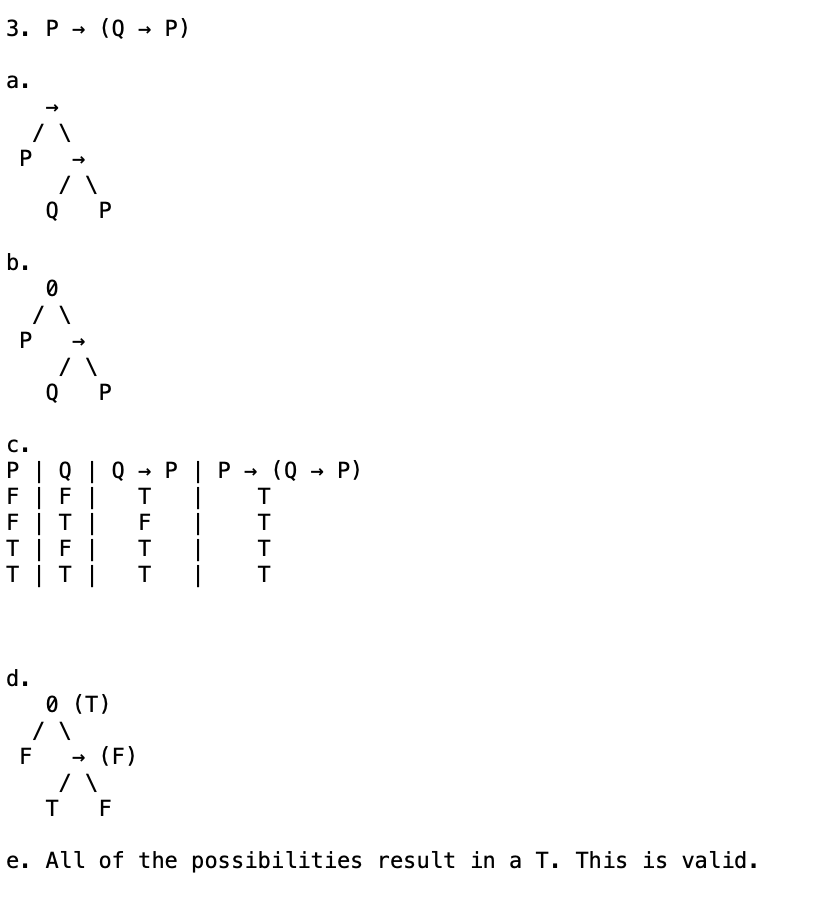
\includegraphics[scale=0.64]{hw6_3}\noindent\newline

\noindent\newline Here is my answer for number 4:

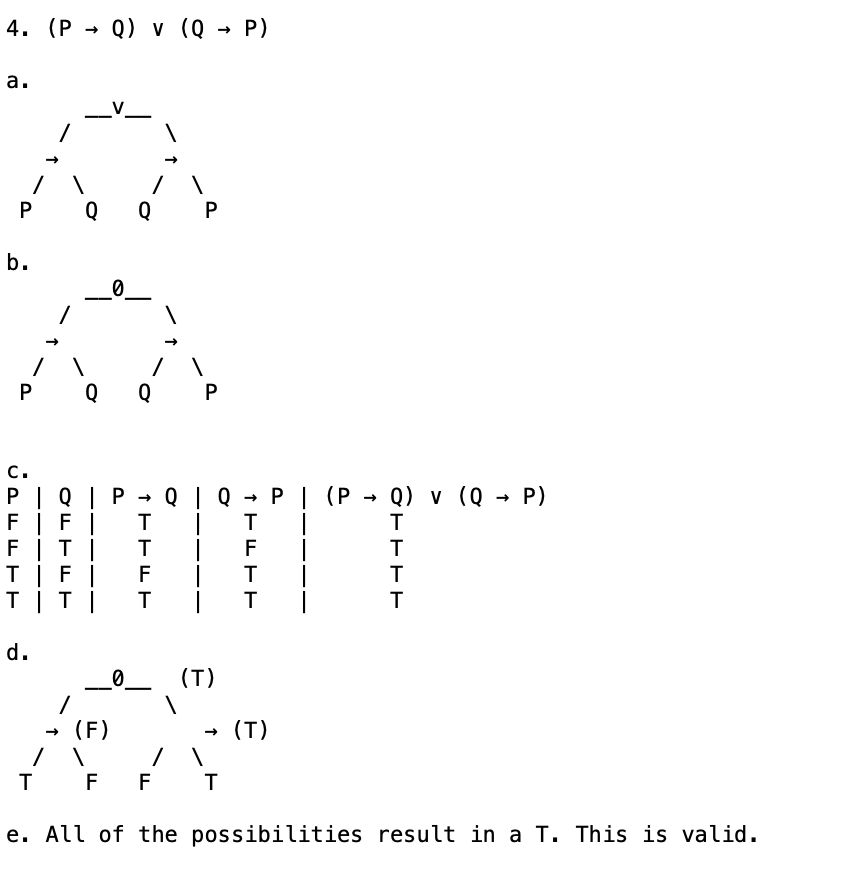
\includegraphics[scale=0.64]{hw6_4}\noindent\newline

\noindent\newline Here is my answer for number 5:

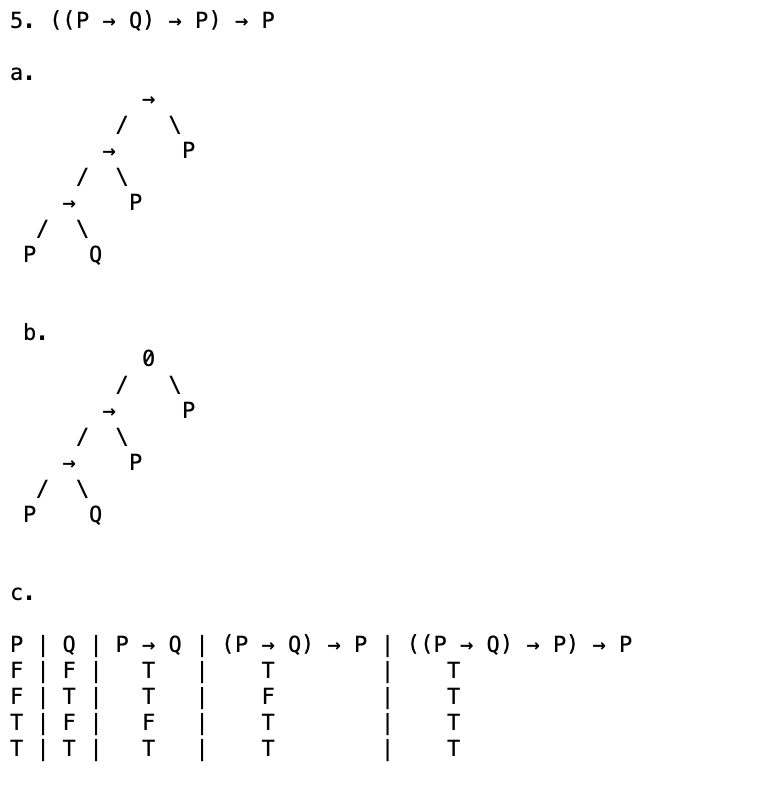
\includegraphics[scale=0.64]{hw6_5_1}\noindent\newline
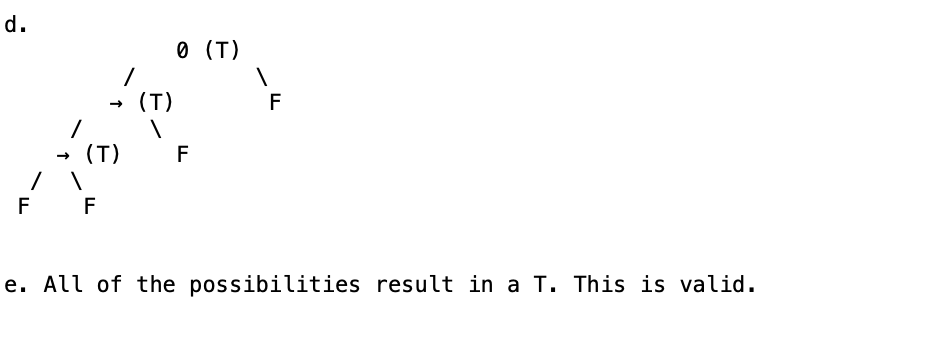
\includegraphics[scale=0.64]{hw6_5_2}\noindent\newline

\noindent\newline Here is my answer for number 6:

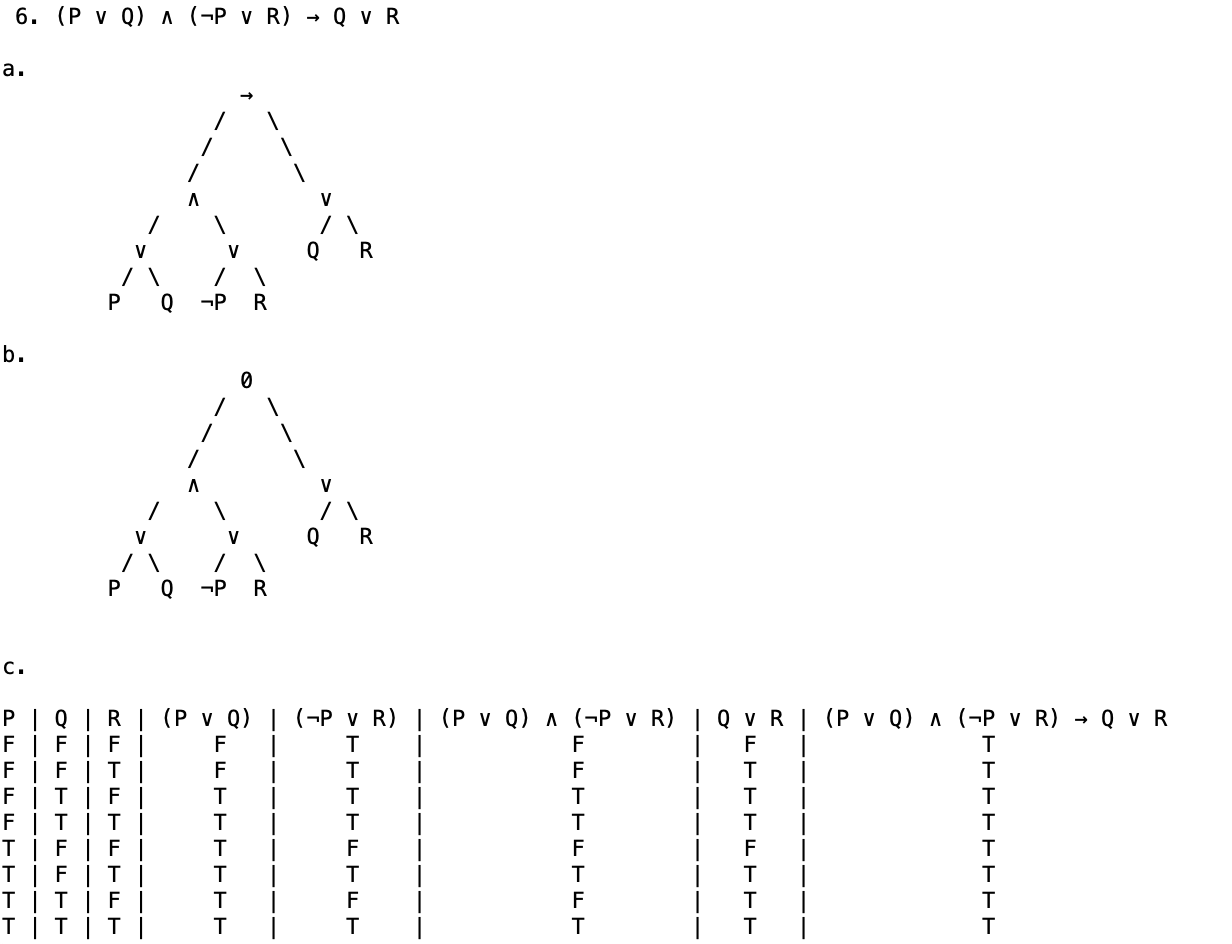
\includegraphics[scale=0.64]{hw6_6}\noindent\newline
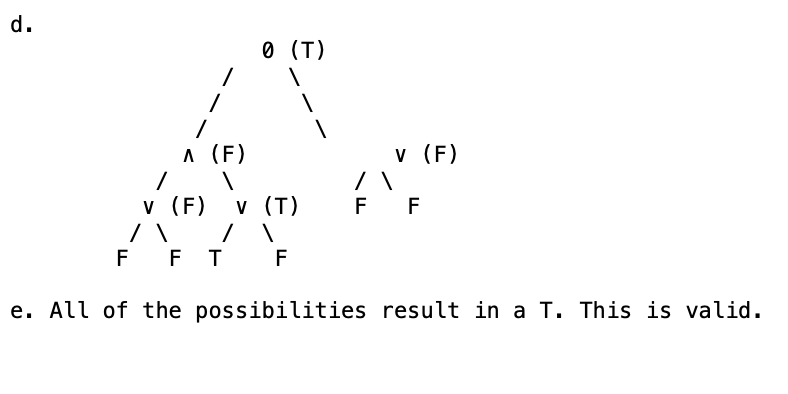
\includegraphics[scale=0.64]{hw6_6_2}\noindent\newline

\subsubsection{Part 1 (Bottom)}
\noindent\newline Here is my answer for number 1:

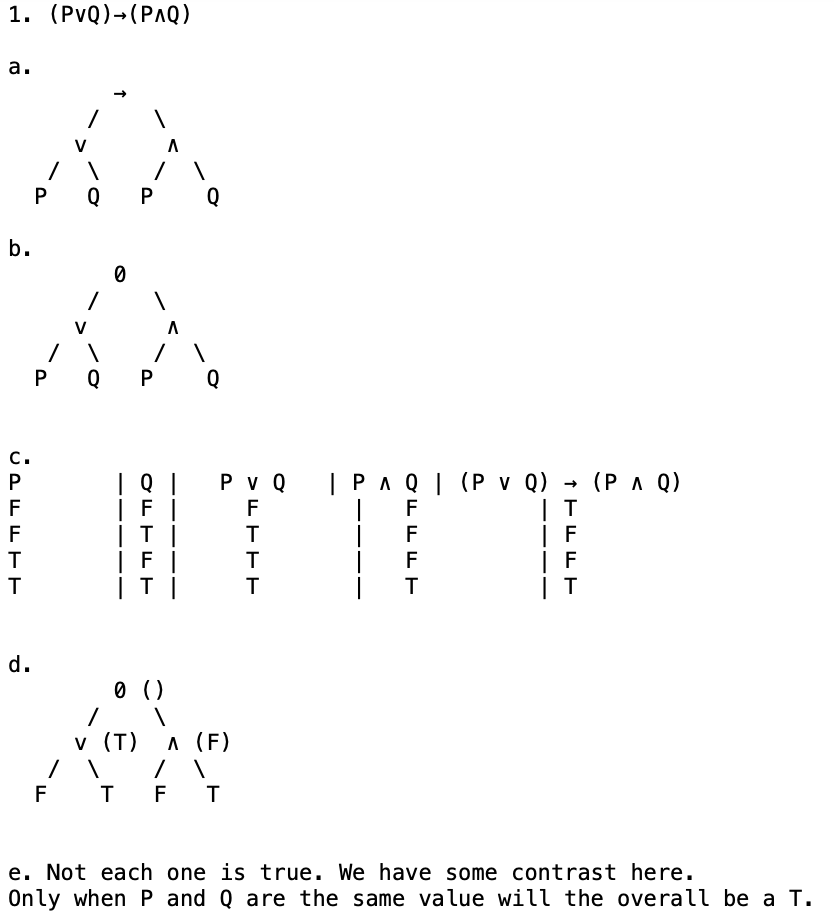
\includegraphics[scale=0.64]{hw6_bottom_1}\noindent\newline

\noindent\newline Here is my answer for number 2:

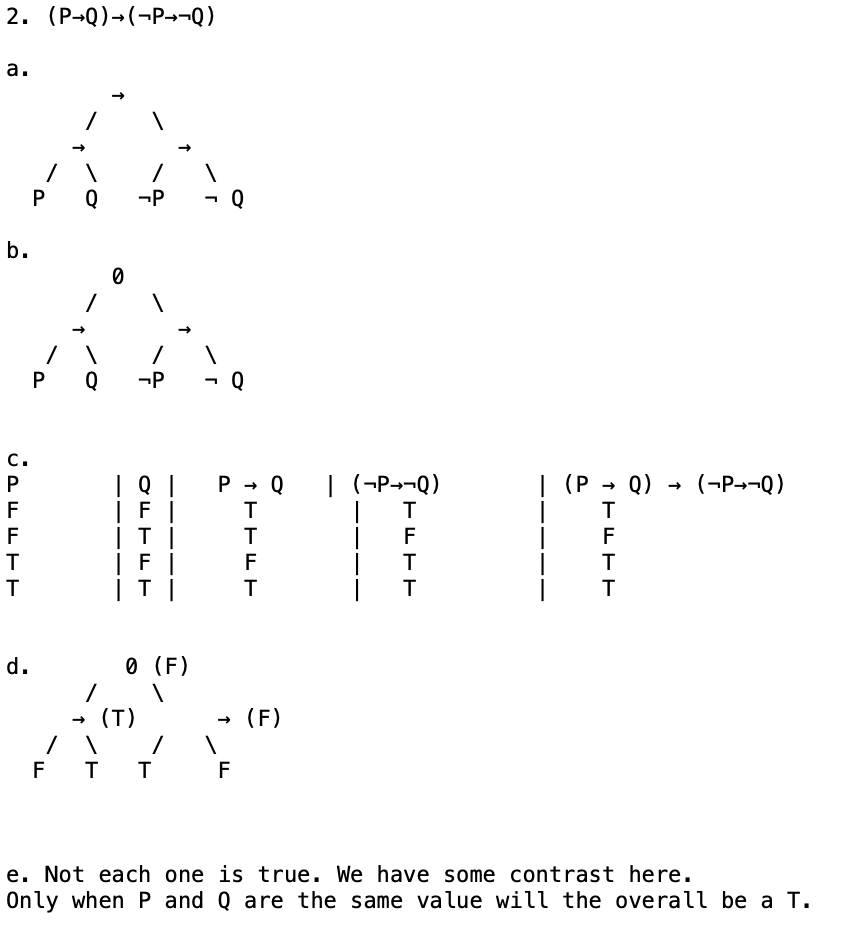
\includegraphics[scale=0.64]{hw6_bottom_2}\noindent\newline


\noindent Note: I had trouble converting some of the symbols I used in my .txt file in my Verbatim. I used many screenshots instead. I will add my .txt and .jpg's in a folder called homeworkMedia on github!

\ldots

\section{Paper}

...

\section{Conclusions}\label{conclusions}

(approx 400 words) A critical reflection on the content of the course. Step back from the technical details. How does the course fit into the wider world of software engineering? What did you find most interesting or useful? What improvements would you suggest?

\begin{thebibliography}{99}
\bibitem[ALG]{Alg} \href{https://github.com/alexhkurz/algorithm-analysis-2023}{Algorithm Analysis}, Chapman University, 2023.
\end{thebibliography}

\end{document}